\documentclass[]{article}
\usepackage[landscape,twocolumn, left=1cm, right=1cm, top=1cm]{geometry}
\usepackage{amssymb}% http://ctan.org/pkg/amssymb
\usepackage[inline]{enumitem}
\usepackage{amsmath}
\usepackage{pgfplots}
\usepackage{multicol}
\begin{document}


\newtheorem{definition}{Definition}
\newtheorem{satz}{Satz}

\section{Algebraische Strukturen}

\section{Matrizen und LGS}

\section{Vektorräume}

\section{Linearkombinationen und Basen}

\section{Lineare Abbildungen}

\section{Darstellungsmatrizen}

\section{Determinanten}

\section{Eigenwerte und Eigenvektoren}

\section{Skalarprodukt}

\pagebreak

\section{Symmetrische Matrizen}

\pagebreak


\section{Relle Zahlen}

\begin{definition}
	Eine Menge $A$ heißt \emph{abzählbar}, falls es eine surjektive Abbildung $f : \mathbb{N} \rightarrow A $ gibt.
\end{definition}

\begin{definition}
	Die reellen Zahlen sind angeordnet, d.h. es gibt ein Prädikat $a > 0$ sodass
	\begin{enumerate}[noitemsep]
		\item $\forall a \in \mathbb{R}$ gilt genau einer der Aussagen $a = 0, a < 0, -a < 0$
		\item $\forall a,b \in \mathbb{R}$ mit $a > 0, b > 0$ gilt: $a + b > 0, a \cdot b > 0$
	\end{enumerate}
\end{definition}

\begin{definition}
	Folgende Mengen nennen wir Intervalle:
	\begin{align}
		(a,b) &:= \{ x \in \mathbb{R} \medspace | \medspace  a    < x    < b \} & \textnormal{offenes Intervall}       \\
		[a,b] &:= \{ x \in \mathbb{R} \medspace | \medspace  a \leq x \leq b \} & \textnormal{geschlossenes Intervall} \\
		(a,b] &:= \{ x \in \mathbb{R} \medspace | \medspace  a    < x \leq b \} & \textnormal{halboffenes Intervall}   \\
		[a,b) &:= \{ x \in \mathbb{R} \medspace | \medspace  a \leq x    < b \} & \textnormal{halboffenes Intervall}	
	\end{align}
\end{definition}

\begin{definition}
	Eine Menge $M \subseteq \mathbb{R}$ heißt \emph{beschränkt}, wenn
	\begin{enumerate}[noitemsep]
		\item $\exists s_0 \in \mathbb{R} : \forall a \in M : a \leq s_0$; $s_0$ heißt \emph{Obere Schranke}
		\item Ist $s_0$ zusätzlich die kleinste obere Schranke, so heißt $s_0$ \emph{Supremum}
		\item $\exists s_0 \in \mathbb{R} : \forall a \in M : s_0 \leq a$; $s_0$ heißt \emph{Untere Schranke}
		\item Ist $s_0$ zusätzlich die größte untere Schranke, so heißt $s_0$ \emph{Infimum}
	\end{enumerate}
\end{definition}

\begin{satz}[Supremumsaxiom]
	Es gilt:
	\begin{enumerate}[noitemsep]
		\item Jede nichtleere nach oben beschränlte Menge $M \subseteq \mathbb{R}$ besitzt ein Supremum, $sup(M) \in \mathbb{R}$
		\item Jede nichtleere nach unten beschränlte Menge $M \subseteq \mathbb{R}$ besitzt ein Infimum, $inf(M) \in \mathbb{R}$
		\item $sup(M) \in M \rightarrow sup(M)$ heißt auch Maximum von $M$
		\item $inf(M) \in M \rightarrow inf(M)$ heißt auch Minimum von $M$
	\end{enumerate}
\end{satz}

\begin{satz}[Archimedizität]
	$\mathbb{R}$ ist archimedisch, d.h. $\forall a \in \mathbb{R} : \exists n \in \mathbb{N} : a < n $. Jede relle Zahl besitzt also ein natürliches Supremum. Insbesondere gilt auch (offensichtlich, aber für Konvergenzbeweise hilfreich): $\frac{1}{n} < a$.
\end{satz}

\begin{satz}[Abschätzungen]
	Es gelten die folgenden Abschätzungen:
	
	\begin{enumerate}[noitemsep]
		\item \textbf{\emph{Dreiecksungleichung:}} $\forall x, y \in \mathbb{R} : | x + y | \leq |x| + |y|$
		\item \textbf{\emph{Umgekehrte Dreiecksungleichung:}} 	$\forall x, y \in \mathbb{R} : | x + y | \geq ||x| - |y||$
		\item \textbf{\emph{Cauchy-Schwarz-Ungleichung:}} 	$\forall x, y \in \mathbb{R}^n : | <x + y> | \leq ||x|| + ||y||$
		\item \textbf{\emph{Abschätzen von Polynomen}} 	$ax^2 + bx + c \leq (a + b + c)x^2 $
		\item \textbf{\emph{Abschätzen der Wurzel:}} 	$\sqrt{ab} \leq \frac{a + b}{2}$
		\item \textbf{\emph{Bernoulli-Ungleichung:}} 	$(1+x)^n \geq 1 + nx$ für $x > -1$	
	\end{enumerate}
	
\end{satz}

\begin{satz}[Binomischer Lehrsatz]
	$\sum_{k=0}^{n} \binom{n}{k}a^k b^{n-k} = (a+b)^n$ 
\end{satz}

\section{Folgen}

\begin{definition}
	Eine Folge reeller Zahlen ist eine Abbildung $\mathbb{N} \rightarrow \mathbb{R} : n \rightarrow a_n$. $(a_n)_{n \in \mathbb{N}}$ beschreibt dabei die Folge, $a_n$ einen Folgenindex
\end{definition}


\begin{definition}
	Eine Folge $(a_n)_{n \in \mathbb{N}}$ konvergiert gegen $a \in \mathbb{R}$ genau dann wenn \\ $\forall \epsilon > 0 : \exists n_0 \in \mathbb{N} : \forall n \geq n_0 : | a_n - a | < \epsilon$, d.h. egal wie klein $\epsilon$, findet man eine Indexschranke $n_0$ sodass alle Folgeindices $a_n$ einen Abstand zu $a$ kleiner als $\epsilon$ haben. Wir schreiben $\lim_{n \rightarrow \infty} a_n = a$
\end{definition}

\begin{definition}
	Eine Folge $(a_n)_{n \in \mathbb{N}}$ divergiert, wenn sie nicht konvergiert. Sie konvergiert zusätzlich uneigentlich gegen
	\begin{enumerate}[noitemsep]
		\item $+ \infty$ genau dann wenn $\forall k > 0 : \exists n_0 \in \mathbb{N} : \forall n \geq n_0 : a_n \geq k$, d.h. ab einen Index sind all $a_n \geq k$
		\item $- \infty$ genau dann wenn $\forall k > 0 : \exists n_0 \in \mathbb{N} : \forall n \geq n_0 : a_n \leq -k$, d.h. ab einen Index sind all $a_n \leq -k$		
	\end{enumerate}
\end{definition}

\begin{definition}
	Eine Folge $(a_n)_{n \in \mathbb{N}}$ heißt \emph{beschränkt}, falls $\exists c > 0 : \forall n \in \mathbb{N} : a_n \leq c$
\end{definition}

\begin{satz}[Rechenregeln für Grenzwerte]
	Falls $\lim_{n \rightarrow \infty} a_n = a \in \mathbb{R}$ sowie \\ $\lim_{n \rightarrow \infty} b_n = b \in \mathbb{R}$, gilt:
	\begin{enumerate}[noitemsep]
		\item $\lim_{n \rightarrow \infty} (a_n \pm b_n) = \lim_{n \rightarrow \infty} a_n \pm \lim_{n \rightarrow \infty} b_n = a \pm b $
		\item $\lim_{n \rightarrow \infty} c \cdot a_n = c \cdot \lim_{n \rightarrow \infty} a_n = c \cdot a  $
		\item $\lim_{n \rightarrow \infty} a_nb_n = \lim_{n \rightarrow \infty} a_n \cdot \lim_{n \rightarrow \infty} b_n = ab  $
		\item $b \neq 0 \rightarrow\lim_{n \rightarrow \infty} \frac{a_n}{b_n} = \frac{\lim_{n \rightarrow \infty} a_n}{\lim_{n \rightarrow \infty} b_n} = \frac{a}{b} $
		\item $\lim_{n \rightarrow \infty} \sqrt{a_n} = \sqrt{a} $
		\item $\lim_{n \rightarrow \infty} |a_n| = |a| $
	\end{enumerate}
\end{satz}

\begin{satz}[Einschließungsregel]
	Es gelte $a_n \leq b_n \leq c_n$ für alle bis auf endlich viele $n$. Falls $\lim_{n \rightarrow \infty} a_n = \alpha$ und $\lim_{n \rightarrow \infty} c_n = \alpha $, dann ist auch $\lim_{n \rightarrow \infty} b_n = \alpha$.
\end{satz}

\begin{definition}[Monotone Folgen]
	Eine Folge $(a_n)_{n \in \mathbb{N}}$ heißt
	\begin{enumerate}[noitemsep]
		\item \emph{monoton fallend}, falls $a_n \geq a_{n+1}$ für alle $a_n$
		\item \emph{monoton steigend}, falls $a_n \leq a_{n+1}$ für alle $a_n$
		\item Gilt sogar $<$ bzw. $>$, so spricht man von \emph{strenger Monotonie}
	\end{enumerate}
\end{definition}

\begin{satz}[Monotonie und Konvergenz]
	Es gilt:
	\begin{enumerate}[noitemsep]
		\item $(a_n)_{n \in \mathbb{N}}$ monoton wachsend $\rightarrow \lim_{n \rightarrow \infty} a_n = sup(a_n)$
		\item $(a_n)_{n \in \mathbb{N}}$ monoton fallend $\rightarrow \lim_{n \rightarrow \infty} a_n = inf(a_n)$
		\item Jede beschränkte monotone Folge konvergiert
		\item Jede unbeschränkte monotone Folge konvergiert uneigentlich gegen $\pm \infty$
	\end{enumerate}
\end{satz}

\begin{definition}[Asymptotische Gleichheit]
	 $(a_n)_{n \in \mathbb{N}}$,  $(b_n)_{n \in \mathbb{N}}$ heißen asymptotisch gleich, falls $\lim_{n \rightarrow \infty} \frac{a_n}{b_n} = 1$. Man schreibt: $a_n \backsimeq b_n$
\end{definition}

\section{Reihen}


\begin{definition}
	Zu einer Folge $(a_n)_{n \in \mathbb{N}}$ sei $(s_n)_{n \in \mathbb{N}}$ mit $s_n := \sum_{k=0}^{n} a_k$ die Folge der Partialsummen. $\lim_{n \rightarrow \infty} s_n = \lim_{n \rightarrow \infty} \sum_{k=0}^{n} a_k = \sum_{k=0}^{\infty} a_k$ heißt Werte der Reihe. Die Reihe konvergiert, wenn $(s_n)_{n \in \mathbb{N}}$ konvergiert, sonst divergiert sie.
\end{definition}

\begin{satz}[Konvergenzkriterium]
	 $\sum_{k=0}^{\infty} a_k $ konvergiert $\rightarrow \lim_{k \rightarrow \infty} a_k = 0$
\end{satz}

\begin{satz}[Majorantenkriterium]
	Es gilt:
	\begin{enumerate}[noitemsep]
		\item Findet man zur Reihe	$\sum_{k=0}^{\infty} a_k $ eine Reihe $\sum_{k=0}^{\infty} b_k $ sodass $b_k \geq |a_k|$, dann gilt: $\sum_{k=0}^{\infty} b_k$ konvergiert $\rightarrow \sum_{k=0}^{\infty} a_k $ konvergiert. $\sum_{k=0}^{\infty} b_k $ heißt Majorante
		\item Findet man zur Reihe	$\sum_{k=0}^{\infty} a_k $ eine Reihe $\sum_{k=0}^{\infty} b_k $ sodass $|b_k| \leq a_k$, dann gilt: $\sum_{k=0}^{\infty} b_k$ divergiert $\rightarrow \sum_{k=0}^{\infty} a_k $ divergiert. $\sum_{k=0}^{\infty} b_k $ heißt Minorante	
	\end{enumerate}
\end{satz}

\begin{satz}[Konvergenzkriterium]
	Sind die Folgen $(a_n)_{n \in \mathbb{N}}$ und $(b_n)_{n \in \mathbb{N}}$ asymptotisch gleich, dann sind $\sum_{k=0}^{\infty} a_k$ und $\sum_{k=0}^{\infty} b_k$ entweder beide konvergent oder beide divergent.
\end{satz}

\begin{satz}[Quotientenkriterium]
	Sei $a_k \neq 0$ bis auf endlich viele $k$. Dann gilt:
	\begin{equation}
		\lim_{k \rightarrow \infty} | \frac{a_{k + 1}}{a_k} | = 
		\begin{cases}
		< 1 & \rightarrow \sum_{k=0}^{\infty} a_k \medspace \textnormal{ist konvergent} \\ 
		> 1 & \rightarrow \sum_{k=0}^{\infty} a_k \medspace \textnormal{ist divergent}  \\
		= 1 & \rightarrow \textnormal{keine Aussage möglich}
		\end{cases}
	\end{equation}
\end{satz}

\begin{satz}[Leibnizkriterium]
	Sei $(a_k)_{k \in \mathbb{N}}$ monoton fallend und $\lim_{k \rightarrow \infty} a_k = 0$. Dann ist $\sum_{k=0}^{\infty} (-1)^k a_k$ konvergent.
\end{satz}

\begin{definition}
	$\sum_{k=0}^{\infty} a_k$ ist absolut konvergent, wenn 	$\sum_{k=0}^{\infty} | a_k | $ konvergiert.
\end{definition}

\begin{satz}[Integralkriterium]
	Sei $f : [1,\infty] \rightarrow [0, \infty]$ monoton fallend. 	$\sum_{k=1}^{\infty} f(k) $ konvergiert $\leftrightarrow \int_{1}^{\infty} f(x) \medspace dx $ konvergiert
\end{satz}

\begin{satz}[Rechenregeln für konvergente Reihen]
	Sind $\sum_{k=1}^{\infty} a_k$ und $\sum_{k=1}^{\infty} b_k$ konvergente Reihen, dann gilt:
	\begin{enumerate}[noitemsep]
		\item \emph{\textbf{Summe konvergenter Reihen:}} $\sum_{k=0}^{\infty} a_k + \sum_{k=0}^{\infty} b_k = \sum_{k=0}^{\infty} (a_k + b_k)$
		\item \emph{\textbf{Multiplikation mit einer Konstante:}} $c \cdot \sum_{k=0}^{\infty} a_k = \sum_{k=0}^{\infty} c \cdot a_k$
		\item \emph{\textbf{Cauchy-Produkt:}} Sind beide Reihen absolut konvergent, dann auch $\sum_{k=0}^{\infty} c_k$, wobei $c_k = \sum_{l=0}^{\infty} a_lb_{k-l}$
		\item \emph{\textbf{Divergente Teilsumme:}}  Ist $\sum_{k=0}^{\infty} b_k$ divergent, dann auch $\sum_{k=0}^{\infty} (a_k + b_k) $
	\end{enumerate}
\end{satz}

\begin{satz}[Bekannte Reihen]
	Folgende Reihen sind zu merken:
	\begin{enumerate}[noitemsep]
	\item \emph{\textbf{Harmonische Reihe:}} $\sum_{k=1}^{\infty} \frac{1}{k} = \infty$ (Divergenz)
	\item \emph{\textbf{Geometrische Reihe:}} $\sum_{k=0}^{\infty} z^k = \frac{1}{1 - z}$, falls $|z| < 1$
	\item \emph{\textbf{Teleskopreihe Reihe:}}  $\sum_{k=1}^{\infty} \frac{1}{k(k+1)} = 1$
	\item \emph{\textbf{Riemannsche Zetafunktion:}} $\zeta(s) = \sum_{k=1}^{\infty} \frac{1}{k^s}$ ist konvergent für $s>1$	
	\item \emph{\textbf{Exponentialreihe:}} $e^x = \sum_{k=0}^{\infty} \frac{x^k}{k!}$ konvergiert	
\end{enumerate}
\end{satz}

\section{Stetigkeit}
\begin{definition}
	Für eine Funktion $f : \mathbb{R} \rightarrow \mathbb{R}$ definiert man $\lim_{x \rightarrow \infty} f(x) = b \in \mathbb{R} \cup \{\pm \infty\}$, wenn für jede relle Folge $(x_n)_{n \in \mathbb{N}}$ mit $\lim_{n \rightarrow \infty} = + \infty$ gilt, dass $\lim_{n \rightarrow \infty} f(x_n) = b$ ist. Analog gilt dies für $- \infty$
\end{definition}

\begin{definition}[Stetigkeit]
	Eine Funktion $f : D \rightarrow \mathbb{R}$ heißt im Punkt $x \in D$ stetig, falls für alle Folgen $(x_n)_{n \in \mathbb{N}}$ in $D$ mit $\lim_{n \rightarrow \infty} x_n = x$ gilt: $\lim_{n \rightarrow \infty} f(x_n) = f(x)$. Man schreibt dann auch $\lim_{y \rightarrow x} f(y) = f(x)$. $f$ ist stetig auf $D$, wenn $f$ in jedem $x \in D$ stetig ist. 
\end{definition}

\begin{definition}[Rechts-/Linksseitiger Grenzwert]
	Man schreibt $\lim_{x \uparrow x_0} f(x) = c$, wenn für jede Folge $(x_n)_{n \in \mathbb{N}}$ mit $x_n > x_0$ für alle $n$ und $\lim_{n \rightarrow x_n} = x_0$ gilt, dass $\lim_{n \rightarrow \infty} f(x_n) = c$. Man spricht vom \emph{Rechtsseitigem Grenzwert}. Analog definiert man den \emph{linksseitigen Grenzwert}.
\end{definition}

\begin{satz}[Rechenregeln stetiger Funktionen]
	Summen und Produkte stetiger Funktionen sind stetig. Die Komposition stetiger Funktionen ist stetig. Polynome und rationale Funktionen sind stetig. Die Betragsfunktion, Wurzelfunktion und die Exponentialfunktion sind stetig.
\end{satz}

\begin{satz}[Zwischenwertsatz]
	Sei $f:[a,b] \rightarrow \mathbb{R}$ stetig. Sei $y \in \mathbb{R}$ und $f(a) < y < f(b)$ oder $f(b) < y < f(a)$. Dann gilt: $\exists x \in (a,b) : f(x) = y$
\end{satz}

\begin{satz}
	Sei $(n_k)_{k \in \mathbb{N}}$ eine streng monoton wachsende Folge in $\mathbb{N}$. Dann heißt  $(a_{n_k})_{k \in \mathbb{N}}$ \emph{Teilfolge} von $(a_n)_{n \in \mathbb{N}}$. $a^*$ heißt \emph{Häufungspunkt} der Folge  $(a_n)_{n \in \mathbb{N}}$, falls es eine Teilfolge  $(a_{n_k})_{k \in \mathbb{N}}$ mit $\lim_{k \rightarrow \infty} a_{n_k} = a^*$ gibt.
\end{satz}

\begin{satz}[Bolzano-Weierstrass]
	Jede beschränkte Folge in $\mathbb{R}$ besitzt mindestens eine konvergente Teilfolge und damit einen Häufungspunkt.
\end{satz}

\begin{definition}
	Eine Menge $A \subseteq \mathbb{R}$ heißt abgeschlossen, wenn für jede Folge $(x_n)_{n \in \mathbb{N}}$ in $A$ gilt: $\lim_{n \rightarrow \infty} x_n = x \rightarrow x\in A$. Eine Menge $K \subseteq \mathbb{R}$ heißt kompakt, wenn $K$ abgeschlossen und beschränkt ist. Jede kompakte Menge besitzt ein Minimum und ein Maximum.
\end{definition}

\begin{satz}
	Sei $K \subseteq \mathbb{R}$ kompakt. Jede stetige Funktion $f : K \rightarrow \mathbb{R}$ nimmt auf $K$ ihr Maximum und Minimum an, d.h. $\exists \bar{x}, \underline{x}: \forall x \in K : f(\underline{x}) \leq f(x) \leq f(\bar{x})$. Man schreibt:
	
	\begin{enumerate}[noitemsep]
		\item $\underline{x} = argmin \{ f(x) \} \medspace$, $f(\underline{x}) = min \{f(x)\}$
		\item $\bar{x} = argmax \{ f(x) \} \medspace$, $f(\bar{x}) = max \{f(x)\}$
	\end{enumerate}

	Achtung: $\bar{x}, \underline{x}$ müssen nicht eindeutig sein.
\end{satz}

\pagebreak

 	
\section{Funktionen}

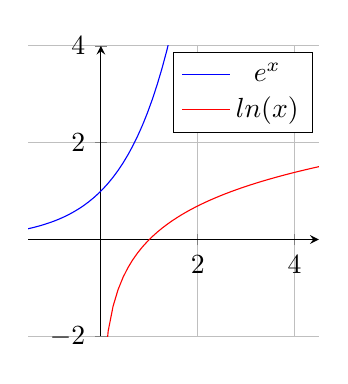
\begin{tikzpicture}
	\begin{axis}[
	width=200,
	height = 150,
	ymin=-2,
	ymax=4,
	xmin=2,
	xmax=1,
	samples=100,
	grid=both,
	no markers,
	axis equal,
	axis x line=center,
	axis y line=center,
	]

		\addplot  {e^x};
		\addlegendentry{$e^x$}
		\addplot {ln (x)};	
		\addlegendentry{$ln (x)$}
	\end{axis}
\end{tikzpicture}

\begin{definition}[Exponentialfunktion]
	$e^x := \lim_{n \rightarrow \infty} (1 + \frac{x}{n})^n = \sum_{k=0}^{\infty} \frac{x^k}{k!}$
	\begin{description} [noitemsep]
		\item Grenzwerte: $\lim_{x \rightarrow \infty} e^x = \infty$, $\lim_{x \rightarrow -\infty} e^x = 0$, $\lim_{x \rightarrow 0} e^x = 1$
		\item Ableitung: $\frac{\partial}{\partial x}(e^x) = e^x$, $\frac{\partial}{\partial x}(e^{-x}) = -e^{-x}$		
		\item Abschätzung: $ 0 \leq 1 + x \leq e^x$,  $x < 1 \rightarrow e^x \leq \frac{1}{1 - x}$ 
		\item Rechenregeln: $e^x \cdot e^y = e^{x+y}$, $e^x \div e^y = e^{x-y}$
		\item Weitere Eigenschaften: stetig auf $\mathbb{R}$, differenzierbar auf $\mathbb{R}$, streng monoton wachsend, Wertemenge: $(0, \infty)$, $\lim_{x \rightarrow \infty} \frac{e^x}{x^m} = \infty$, $\lim_{x \downarrow 0} \frac{e^x - 1}{x} = 1$
		\item Komplexe Exponentialfunktion: $e^{x+iy} = e^x(cos(y) + i sin(y)) \rightarrow e^{iy} = cos(y) + i sin(y)$
	\end{description}
\end{definition}

\begin{definition}[Logarithmusfunktion]
	$ln(e^x) := x$, $ln : (0, \infty) \rightarrow \mathbb{R}$
	
	\begin{description} [noitemsep]
		\item Grenzwerte: $\lim_{x \rightarrow \infty} ln (x) = \infty$, $\lim_{x \downarrow 0} ln (x )= - \infty$
		\item Ableitung: $\frac{\partial}{\partial x} (ln(x)) = \frac{1}{x}$, $\frac{\partial}{\partial x} (ln(x + a)) = \frac{1}{x + a}$
		\item Abschätzung: für $x > 1$ gilt $1 - \frac{1}{x} < ln(x) < x - 1$
		\item Rechenregeln: $ln(xy) = ln(x) + ln(y)$, $ln(x \div y) = ln(x) - ln(y)$, $ln(x^k) = k \cdot ln(x)$
		\item Weitere Eigenschaften: stetig auf $(0,\infty)$, differenzierbar auf $(0,\infty)$, streng monoton wachsend, Wertemenge: $(- \infty, \infty)$, $\lim_{x \downarrow 0} x \cdot ln(x) = 0$, $\lim_{x \mapsto \infty} \frac{x}{ln(x)^n} = \infty$,  $\lim_{x \rightarrow \infty} \frac{ln(x)}{ln(ln(x))} = \infty$,  $\lim_{x \downarrow 0} \frac{ln(1+x)}{x} = 1$
	\end{description}
\end{definition}

\begin{definition}[Allgemeine Logarithmus - und Potenzfunktion]
 $\medspace$	\\ $x > 0, a \in \mathbb{R}$ : $x^a = e^{ln(x^a)} = e^{a ln(x)}$ \\ $b^x = y \leftrightarrow x = log_b \leftrightarrow y = \frac{ln (y)}{ln(b)}$
	\begin{description} [noitemsep]
		\item Grenzwerte: $\lim_{x \rightarrow \infty} x^a = \begin{cases}
		+ \infty & a > 0 \\ 
		1        & a = 0  \\
		0        & a < 0
		\end{cases} \medspace \medspace $,
		$\lim_{x \downarrow 0} x^a = \begin{cases}
		0        & a > 0 \\ 
		1        & a = 0  \\
		+ \infty & a < 0
		\end{cases}$,\\
		 $\lim_{x \rightarrow \infty} \frac{x^a}{b^x} = 0$, $a > 0 \rightarrow \lim_{x \downarrow 0} x^a ln(x) = 0$, $\lim_{x \downarrow 0} \frac{ln(1+x)}{x} = 1$
		\item Ableitung: $\frac{\partial}{\partial x} (x^a) = a x^{a - 1}$, $\frac{\partial}{\partial x}(b^x) = ln(x) \cdot b^x$
		\item Rechenregeln: $x^{\frac{m}{n}} = \sqrt[m]{x^n} = (\sqrt[m]{x})^n$
	\end{description}
\end{definition}

\pagebreak

\section{Trigonometrische Funktionen}

\begin{definition}[Einheitskreis]
Sinus und Kosinus beschreiben die Länge der Ankathete bzw. Gegenkathete im Einheitskreis.

\begin{multicols}{2}
	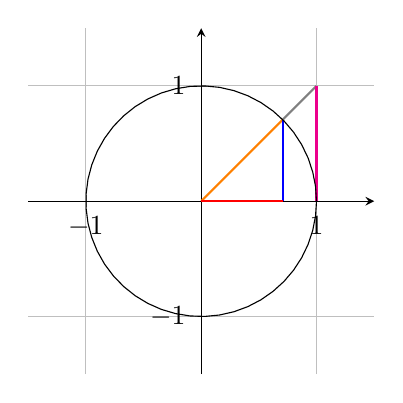
\begin{tikzpicture}
	\begin{axis}[
		width=170,
		height = 170,
		ymin=-1.5,
		ymax=1.5,
		xmin=-1.5,
		xmax=1.5,
		samples=100,
		grid=both,
		no markers,
		axis x line=center,
		axis y line=center,
	]
		\addplot [thick, orange, domain=0:0.707]{x)};
		\addplot [thick, blue] coordinates {(0.707,0)(0.707,0.707)};
		\addplot [thick, domain=0:0.707, red]{0};
		\addplot [thick, gray, domain=0.707:1]{x)};
		\addplot [thick, magenta] coordinates {(1,0)(1,1)};		
		\addplot [domain=0:2*pi,samples=50]({cos(deg(x))},{sin(deg(x))});
	\end{axis}
	\end{tikzpicture}
	\begin{itemize}[label={}, noitemsep]
		\item \textcolor{red}{Ankathete(x)} $= cos(x)$
		\item \textcolor{blue}{Gegenkathete(x)} $= sin(x)$
		\item \textcolor{orange}{Hypthenuse(x)} $= 1 \overset{\text{Pythagoras}}{=} cos(x)^2 + sin(x)^2$	
		\item \textcolor{magenta}{Tangente(x)} $= tan(x)$			
		\item $\pi := \frac{\textnormal{Kreisumfang U}}{\textnormal{Durchmesser d}} \overset{\text{Einheitskreis}}{=} \frac{U}{2} \leftrightarrow 2 \pi = U $
		\item $\rightarrow$ Kosinus und Sinus sind $2 \pi$ periodisch
		\item $\rightarrow cos(2 \pi x) = cos(x)$, $sin(2 \pi x) = sn(x)$
	\end{itemize}
\end{multicols}



\end{definition}

\begin{definition}[Analytisch]
	Analytische Definition
	\begin{multicols}{2}
		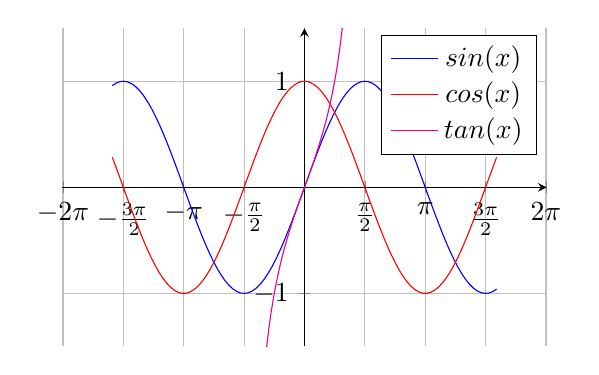
\begin{tikzpicture}
		\begin{axis}[
		width=220,
		height = 160,
		ymin=-1.5,
		ymax=1.5,
		xmin=-6.3,
		xmax=6.3,
		samples=100,
		grid=both,
		no markers,
		axis x line=center,
		axis y line=center,
		    xtick={
			-6.28318, -4.7123889, -3.14159, -1.5708,
			1.5708, 3.14159, 4.7123889, 6.28318
		},
		    xticklabels={
			$-2\pi$, $-\frac{3\pi}{2}$, $-\pi$, $-\frac{\pi}{2}$,
			$\frac{\pi}{2}$, $\pi$, $\frac{3\pi}{2}$, $2\pi$
		}
		]
		\addplot  {sin (deg(x))};
		\addlegendentry{$sin (x)$}
		\addplot {cos (deg(x))};	
		\addlegendentry{$cos (x)$}
		\addplot [magenta, domain=-1.5:1.5]{tan (deg (x)};
		\addlegendentry{$tan (x)$}
		\end{axis}
		\end{tikzpicture}
		
		\begin{itemize}[label={}, noitemsep]
			\item $sin(x)  = \sum_{k = 0}^{\infty} (-1)^k \cdot \frac{x^{2k+1}}{(2k +1)!} \overset{\text{Euler}}{=} \frac{1}{2i}(e^{ix} - e^{-ix})$ 
			\item $cos(x)  = \sum_{k = 0}^{\infty} (-1)^k \cdot \frac{x^{2k}}{(2k)!}      \overset{\text{Euler}}{=} \frac{1}{2} (e^{ix} + e^{-ix})$
			\item $\rightarrow cos(x) = sin(x + \frac{\pi}{2})$, $sin(x) = cos(x - \frac{\pi}{2})$ 	
			\item $tan : (- \frac{\pi}{2}, \frac{\pi}{2}) \rightarrow (-\infty, \infty) : x \rightarrowtail \frac{sin(x)}{cos(x)}$
	\end{itemize}
		
	\end{multicols}
\end{definition}

\begin{definition}[Eigenschaften]
	Für Sinus, Kosinus und Tangens gilt:
	\begin{description}[noitemsep]
		\item $sin(0) = 0, sin( \frac{\pi}{2})=1, sin(\pi) = 0, sin(\frac{3 \pi}{2}) = -1, sin(2 \pi) = 0$
		\item $cos(0) = 1, cos (\frac{\pi}{2}) = 0, cos (\pi) = 1, cos(\frac{3 \pi}{2}) = 0, cos (2 \pi) = 1$
		\item $tan(0) = 0, tan(\pi) = 0, tan(2 \pi) = 0 \dots$
		\item Ableitung: $\frac{\partial}{\partial x}(cos(x)) = -sin(x), \frac{\partial}{\partial x}(sin(x)) = cos(x)$, \\ $\frac{\partial}{\partial x}(tan(x)) = \frac{1}{cos(x)^2} = 1 + tan(x)^2$
		\item Grenzwerte $\lim_{x \rightarrow 0} \frac{sin(x)}{x} = 1, \lim_{x \rightarrow 0} \frac{1 - cos(x)}{0.5x} = 1, \lim_{x \downarrow 0} \frac{tan (x)}{x} = 1$
		\item Rechenregeln: $cox(-x) = cos(x), sin(-x) = -sin(x)$ \\ $cos(x \pm y) = cos(x)cos(y) \pm sin(x)sin(y)$, \\ $sin(x \pm y) = sin(x)cos(y) \pm sin(y)cos(x)$
		\item Weitere Eigenschaften: stetig und differenzierbar auf dem gesamten Definitionsbereich
	\end{description}
\end{definition}

\pagebreak

\begin{definition}[Umkehrfunktionen]
Für Sinus, Kosinus und Tangens seien die folgenden Umkehrfunktionen definiert:
	\begin{multicols}{2}
		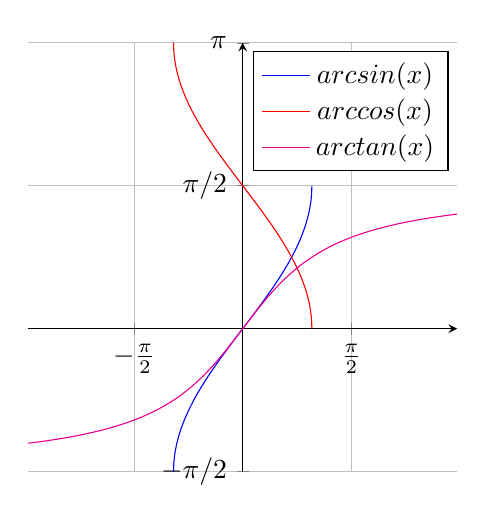
\begin{tikzpicture}
			\begin{axis}[
			width=200,
			height = 200,
			domain=-3.1:3.1, 
			samples=500, 
			axis x line=center,
			axis y line=center,
			xtick={-3.14,-1.57,0,1.57,3.14}, 
			ytick={-1.57,1.57,3.14}, 
			xticklabels={$-\pi$, $-\frac{\pi}{2}$, $0$, $\frac{\pi}{2}$, $\pi$},
			yticklabels={$-\pi$/2,$\pi$/2,$\pi$},
			grid=both]
			\addplot[color = blue,domain=-1:1]  {asin(x)/180*pi};
			\addlegendentry{$arcsin (x)$}
			\addplot[color = red, domain=-1:1]  {acos(x)/180*pi};
			\addlegendentry{$arccos (x)$}
			\addplot[color = magenta]  {atan(x)/180*pi};
			\addlegendentry{$arctan (x)$}
			\end{axis}
		\end{tikzpicture}
		
	
			\begin{description}[noitemsep]
				\item $arcsin : [-1,1] \rightarrow [0, \pi] : x \mapsto sin^{-1}(x) $
				\item $arccos : [-1,1] \rightarrow [-\frac{\pi}{2},\frac{\pi}{2}] : x \mapsto cos^{-1}(x) $
				\item $arctan : \mathbb{R} \rightarrow [-\frac{\pi}{2},\frac{\pi}{2}] : x \mapsto tan^{-1} $
			\end{description}
	
	\end{multicols}
\end{definition}

\section{Komplexe Zahlen}

\begin{definition}
	Als Erweiterung der reellen Zahlen sei definiert:
	\begin{description}[noitemsep]
		\item $z \in \mathbb{C}, z = x + iy$, wobei $x,y \in \mathbb{R}$ und $i := \sqrt{-1} \leftrightarrow i^2 = -1$
		\item $x := Re(z)$ nennt man \emph{Realteil} von $z$, $y := Im(z)$ heißt \emph{Imaginärteil} von $z$
		\item $\bar{z} = z^* := x - iy, |z| = \sqrt{x^2 + y^2}$
		\item $\rightarrow Re(z) = \frac{z + \bar{z}}{2}, Im(z) = \frac{z - \bar{z}}{2}$
	\end{description}
\end{definition}

\begin{definition}[Polardarstellung]
	Anstelle in die Zahleneben $x,y$ einer komplexen Zahl zu verwenden, lässt sich alternativ die Länge $r$ der Zahl sowie der Winkel $\phi$ zur reellen Achse benutzen:
	
	\begin{tikzpicture}
	\begin{axis}[
	ticks=none,
	domain=0:2,
	width=220,
	height=150,
	xmax=1.5,
	ymax=1.25,
	axis x line=center,
	axis y line=center,
	no markers]
	
	\addplot [red, domain=0:1]{x}  node[above,pos=1] {$z = x + iy$};
	\addplot [blue, domain=0:1] coordinates {(1,0)(1,1)};	
	\node[right] at (50, 5)  {$x = r cos(\phi)$} ;
	\node[right] at (15, 50)  {$r = |z|$} ;
	\node[right] at (100, 50)  {$y = r sin(\phi)$} ;
	\node[right] at (15, 10)  {$\phi$} ;
	\end{axis}
	\end{tikzpicture}
\end{definition}

\begin{satz}[Euler'sche Formel]
	$e^{iy} = cos(x) + i sin(x)$
	
	\begin{description}[noitemsep]
		\item $\rightarrow e^{it}$ durchläuft den Einheitskreis 
		\item $\rightarrow e^{i \cdot 0} = e^{i \cdot 2k\pi} = 1, e^{-i\pi} = -1$
	\end{description}
	
\end{satz}


\pagebreak

\section{Differenzierbarkeit}

\begin{definition}[Landau-Symbole]
	Seien $f,g : \mathbb{R} \rightarrow \mathbb{C}$ Funktionen, $x_0 \in \mathbb{R}$
	\begin{description}[noitemsep]
		\item $f(x) = \mathcal{O}(g(x))$ für $x \rightarrow x_0$ falls: $\exists \epsilon > 0: \exists c > 0 : \forall x \in \mathbb{R}$ mit $|x - x _0| < \epsilon : |f(x)| < c \cdot |g(x)|$, d.h. in einer Umgebung von $x_0$ wird $f(x)$ von $g(x)$ mal einer Konstante beschränkt.
		\item $f(x) = o(g(x))$ für $x \rightarrow x_0$ falls $\lim_{x \rightarrow x_0} \frac{f(x)}{g(x)} = 0 $
		\item $f(x) = \mathcal{O}(g(x))$ für $x \rightarrow \infty$ falls: $\exists M > 0: \exists c > 0 : \forall x > M : |f(x)| < c \cdot |g(x)|$, d.h. ab einer Schranke $M$ wird $f(x)$ durch $g(x)$ beschränkt.
		\item $f(x) = \mathcal{O}(g(x))$ für $x \rightarrow -\infty$ falls: $\exists M > 0: \exists c > 0 : \forall x < -M : |f(x)| < c \cdot |g(x)|$, d.h. ab einer Schranke $M$ wird $f(x)$ durch $g(x)$ beschränkt.	
		\item $f(x) = o(g(x))$ für $x \rightarrow x_0 \in \{\pm \infty\}$ falls $\lim_{x \rightarrow x_0} \frac{f(x)}{g(x)} = 0 $
	\end{description}
\end{definition}

\begin{definition}[Differenzierbarkeit]
	Eine Funktion $f : I \rightarrow \mathbb{R}, I \subseteq \mathbb{R}$ heißt differenzierbar in $x_0 \in I$, falls $\lim_{x \rightarrow x_0} \frac{f(x) - f(x_0)}{x - x_0}$ bzw. $\lim_{h \rightarrow 0} \frac{f(x_0 + h) - f(x_0)}{h}$ existiert. Man schreibt dafür $f'(x_0)$ (Lagrange), $\frac{\partial f}{\partial x_0}$ (Leibniz). Ist $f$ differenzierbar für alle $x_0 \in I$, so heißt $f$ differenzierbar.
\end{definition}

\begin{satz}[Rechenregeln differenzierbrer Funktionen]
	Seien $f,g : I \subseteq \mathbb{R} \rightarrow \mathbb{R}$ in $x \in I$ differenzierbar, $c \in \mathbb{R}$.
	\begin{description}[noitemsep]
		\item $(c \cdot f)'(x) = c \cdot f'(x) $
		\item $(f + g)'(x) = f'(x) + g'(x) $
		\item $(f \cdot g)'(x) = f'(x) g(x) + f(x)g'(x) $  (Produktregel)
		\item $(\frac{f}{g})'(x) = \frac{f'(x) g(x) - f(x)g'(x)}{g(x)^2} $	 (Quotientenregel)
	\end{description}
\end{satz}

\begin{satz}[Kettenregel]
	Sei $f : D \subseteq \mathbb{R} \rightarrow \mathbb{R}$, $g : E \subseteq \mathbb{R} \rightarrow \mathbb{R}$ und $g(E) \subseteq D$. Sei $x_0$ innererer Punkt von $E$, $g(x_0)$ innerer Punkt von $D$. Sei $g$ in $x_0$ und $f$ in $g(x_0)$ differenzierbar. Dann gilt: $(f \circ g)'(x_0) = f'(g(x_0)) \cdot g'(x_0)$
 \end{satz}

\begin{satz}[Ableitung der Umkehrfunktion]
	Sei $f : I \subseteq \mathbb{R} \rightarrow J \subseteq \mathbb{R}$ bijektiv und differenzierbar in $y_0$. Dann ist $f^{-1} : J \rightarrow I$ differenzierbar in $y_0$ und $(f^{-1})'=\frac{1}{f'(f^{-1}(y_0))}$
\end{satz}

\begin{satz}[Elementare Ableitungen]
	Es gelten folgende Ableitungen:
	\begin{multicols}{2}
		\begin{description}[noitemsep]
			\item $(c)' = 0$
			\item $(x^a)'=ax^{a-1}$
			\item $(e^x)'=e^x$
			\item $sin'(x) = cos(x)$
			\item $cos'(x) = -sin(x)$
			\item $tan'(x) = \frac{1}{cos(x)^2 = 1 + tan(x)^2}$
			\item $ln'(x) = \frac{1}{x}$
			\item $arcsin'(x) = \frac{1}{\sqrt{1 -x^2}}$	
			\item $arccos'(x) = - \frac{1}{\sqrt{1 - x^2}}$	
			\item $arctan'(x) = \frac{1}{1 + x^2}$
			\item $(a^x)' = a^x ln(a)$
		\end{description}
	\end{multicols}
\end{satz}

\section{Anwendungen der Ableitung}

\begin{satz}
	Sei $f : [a,b] \rightarrow \mathbb{R}$ differenzierbar auf $(a,b)$. Wenn $f$ in $x_0$ ein lokales Extremum besitzt, dann gilt $f'(x_0) = 0$.
\end{satz}

\begin{satz}[Mittelwertsatz]
	Sei $f : [a,b] \rightarrow \mathbb{R}$ differenzierbar auf $[a,b]$, differenzierbar auf $(a,b)$. Dann gibt es ein $\xi \in (a,b)$ sodass $\frac{f(b) - f(a)}{b - a} = f'(\xi)$.
\end{satz}

\begin{satz}[Satz von Rolle]
	Gilt neben dem Mittelwertsatz zusätzlich $f(a) = f(b)$, dann gibt es ein $\xi \in (a,b)$ sodass $f'(\xi) = 0$.
\end{satz}

\begin{satz}[Monotonie und Ableitungen]
	\begin{description}[noitemsep]
		\item $\forall x\in(a,b) : f'(x) > 0 \rightarrow f$ ist auf $[a,b]$ streng monoton wachsend
		\item $\forall x\in(a,b) : f'(x) < 0 \rightarrow f$ ist auf $[a,b]$ streng monoton fallend
		\item $\forall x\in(a,b) : f'(x) \geq 0 \rightarrow f$ ist auf $[a,b]$ monoton wachsend
		\item $\forall x\in(a,b) : f'(x) \leq 0 \rightarrow f$ ist auf $[a,b]$ monoton fallend
	\end{description}
\end{satz}

\begin{satz}
	Sei $f : (a,b) \rightarrow \mathbb{R}$ differenzierbar, sei $f'(x_0) = 0, x_0 \in (a,b)$.
	\begin{description}[noitemsep]
		\item $f' \geq 0$ in $(a, x_0)$ und $f' \leq 0$ in $(x_0, b) \rightarrow x_0$ ist globales Maximum
		\item $f' \leq 0$ in $(a, x_0)$ und $f' \geq 0$ in $(x_0, b) \rightarrow x_0$ ist globales Minimum
	\end{description}
\end{satz}

\begin{satz}
	Seien $f,g :(a,b) \rightarrow \mathbb{R}$ differenzierbar und $f' = g'$ auf $(a,b)$. Dann gibt unterscheiden sich $f,g$ nur um eine Konstante, d.h. $\exists c \in \mathbb{R} : f = g + c$ auf $(a,b)$.
\end{satz}

\begin{satz}[L'Hospital]
	Seien $a,b \in \mathbb{R} \cup \{+ \infty, - \infty\}$. Seien $f, g : (a,b) \rightarrow \mathbb{R}$ differenzierbar mit $g'(x) \neq 0$. Sei $x_0 \in (a,b)$ und es gelte:
	\begin{enumerate}[noitemsep]
		\item $\lim_{x \rightarrow x_0} f(x) = 0 = \lim_{x \rightarrow x_0} g(x)$ oder
		\item$\lim_{x \rightarrow x_0} f(x) = \pm \infty = \lim_{x \rightarrow x_0} g(x)$
	\end{enumerate}
	Falls $\lim_{x \rightarrow x_0} \frac{f'(x)}{g'(x)}$ existiert, gilt: $\lim_{x \rightarrow x_0} \frac{f(x)}{g(x)} = \lim_{x \rightarrow x_0} \frac{f'(x)}{g'(x)}$.
\end{satz}

\begin{definition}
	Für zweimal differenzierbares $f : (a,b) \rightarrow \mathbb{R}$ gilt:
	\begin{enumerate}[noitemsep]
		\item $f$ heißt \emph{konvex} $\leftrightarrow f'' \geq 0$ auf $(a,b)$
		\item $f$ heißt \emph{konkav} $\leftrightarrow f'' \leq 0$ auf $(a,b)$		
	\end{enumerate}
\end{definition}

\begin{satz}
	Sei $f : (a,b) \rightarrow \mathbb{R}$ zweimal differenzierbar und $f'(x_0)=0$ und $\exists x_0 \in (a,b) : f'(x_0) = 0$.
	
	\begin{enumerate}[noitemsep]
		\item $f''(x_0) > 0 \rightarrow f$ besitzt in $x_0$ ein striktes lokales Minimum
		\item $f''(x_0) < 0 \rightarrow f$ besitzt in $x_0$ ein striktes lokales Maximum	
	\end{enumerate}
\end{satz}

\begin{satz}[Differenzierbarkeit und Stetigkeit]
	Ist $f$ differenzierbar, so ist $f$ stetig.
\end{satz}

\section{Integrale}

\begin{multicols}{2}
	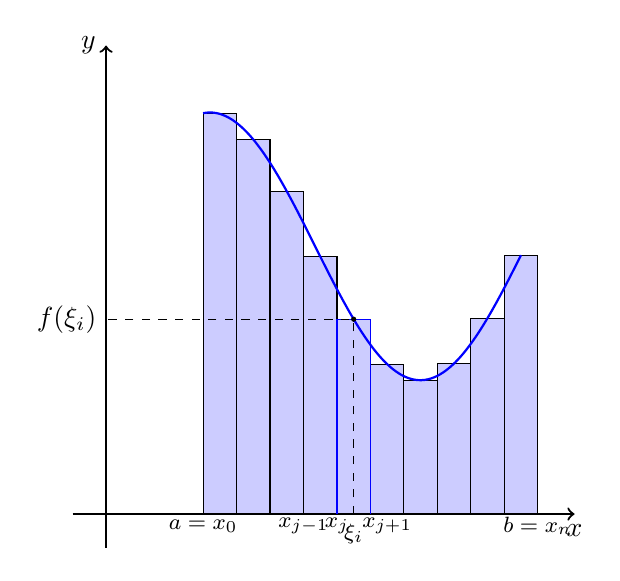
\begin{tikzpicture}[scale=0.85]
	\def\a{1.7}
	\def\b{5.7}
	\def\c{3.7}
	\def\L{0.5} % width of interval
	
	\pgfmathsetmacro{\Va}{2*sin(\a r+1)+4} \pgfmathresult
	\pgfmathsetmacro{\Vb}{2*sin(\b r+1)+4} \pgfmathresult
	\pgfmathsetmacro{\Vc}{2*sin(\c r+1)+4} \pgfmathresult
	
	\draw[->,thick] (-0.5,0) -- (7,0) coordinate (x axis) node[below] {$x$};
	\draw[->,thick] (0,-0.5) -- (0,7) coordinate (y axis) node[left] {$y$};
	\foreach \f in {1.7,2.2,...,6.2} {\pgfmathparse{2*sin(\f r+1)+4} \pgfmathresult
		\draw[fill=blue!20] (\f-\L/2,\pgfmathresult |- x axis) -- (\f-\L/2,\pgfmathresult) -- (\f+\L/2,\pgfmathresult) -- (\f+\L/2,\pgfmathresult |- x axis) -- cycle;}
	\node at (\a-\L/2,-5pt) {\footnotesize{$a=x_0$}};
	\node at (\b+\L/2+\L,-5pt) {\footnotesize{$b=x_n$}};
	\draw[blue] (\c-\L/2,0) -- (\c-\L/2,\Vc) -- (\c+\L/2,\Vc) -- (\c+\L/2,0);
	\draw[dashed] (\c,0) node[below] {\footnotesize{$\xi_i$}} -- (\c,\Vc) -- (0,\Vc) node[left] {$f(\xi_i)$};
	\node at (\a+5*\L/2,-5pt) {\footnotesize{$x_{j-1}$}};
	\node at (\a+7*\L/2,-5pt) {\footnotesize{$x_j$}};
	\node at (\a+5*\L,-5pt) {\footnotesize{$x_{j+1}$}};
	\draw[blue,thick,smooth,samples=100,domain=1.45:6.2] plot(\x,{2*sin(\x r+1)+4});
	\filldraw[black] (\c,\Vc) circle (.03cm);
	\end{tikzpicture}
	
	\begin{definition}[Riemann-Summe]
		Sei $Z$ eine Zerlegung von $[a,b]$ : $a = x_0 < x_1 < \dots < x_{n-1} < x_n = b$. Die Feinheit von $Z$ ist $|Z| = max_{1 \leq j \leq n}\{|x_j - x_{j-1}|\}$. Gegeben sei ein Zerlegung $Z$. Sei $\xi \in [x_{j-1}, x_j]$ mit $1 \leq j \leq n$ beliebig. $S_Z = \sum_{j=1}^{n} f(\xi) \cdot (x_j-x_{j-1})$ heißt Riemann-Summe, wobei $f(\xi)$ Höhe der Rechtecksflächen.
	\end{definition}
\end{multicols}




\section{Potenzreihen}


\section{Mehr über Integrale}


\section{Differentialrechnung mehrerer Veränderlicher}


\section{Gewöhnliche Differentialgleichungen}

\end{document}
